\documentclass[12pt,a4paper]{article}

% Language setting
\usepackage[portuguese]{babel}
%\addto\captionsportuguese{\newcommand{\andname}{e}}

% Set page size and margins
\usepackage[a4paper,top=2cm,bottom=2cm,left=2.5cm,right=2.5cm,marginparwidth=1.75cm]{geometry}


\usepackage{amsmath}
\usepackage{graphicx}
\usepackage[colorlinks=true, allcolors=blue]{hyperref}
\usepackage{hyperref}
\usepackage{orcidlink}
\usepackage[title]{appendix}
\usepackage{mathrsfs}
\usepackage{amsfonts}
\usepackage{booktabs} % For \toprule, \midrule, \botrule
\usepackage{caption}  % For \caption
\usepackage{threeparttable} % For table footnotes
\usepackage{listings}
\usepackage{enumitem}
\usepackage{chngcntr}
\usepackage{booktabs}
\usepackage{lipsum}
\usepackage{subcaption}
\usepackage{authblk}
\usepackage[T1]{fontenc}    % Font encoding
\usepackage{csquotes}       % Include csquotes
\usepackage{diagbox}


% Customize line spacing
\usepackage{setspace}
\onehalfspacing % 1.5 line spacing

% Redefine section and subsection numbering format
\usepackage{titlesec}
\titleformat{\section} % Redefine section numbering format
  {\normalfont\Large\bfseries}{\thesection.}{1em}{}

% Change the position of the table caption above the table
\usepackage{float}   % for customizing caption position
\usepackage{caption} % for customizing caption format
\captionsetup[table]{position=top} % caption position for tables

% Define the unnumbered list
\makeatletter
\newenvironment{unlist}{%
  \begin{list}{}{%
    \setlength{\labelwidth}{0pt}%
    \setlength{\labelsep}{0pt}%
    \setlength{\leftmargin}{2em}%
    \setlength{\itemindent}{-2em}%
    \setlength{\topsep}{\medskipamount}%
    \setlength{\itemsep}{3pt}%
  }%
}{%
  \end{list}%
}
\makeatother

% Suppress the warning about \@parboxrestore
\pdfsuppresswarningpagegroup=1

%-------------------------------------------
% Paper Head
%-------------------------------------------
\title{PTC3314 - Ondas e Linhas}
\author{3º Exercício de Simulação Computacional}

\affil{Guilherme Fortunato Miranda, Nº USP: 13683786}
\affil{João Pedro Dionizio Calazans, Nº USP: 13673086}
\affil{Thomas de Castro Hess, Nº USP: 11806090}
\affil{Turma 02 – Grupo B}

\date{24 de Novembro de 2024}

\begin{document}

\maketitle

\section{}

\begin{center}
    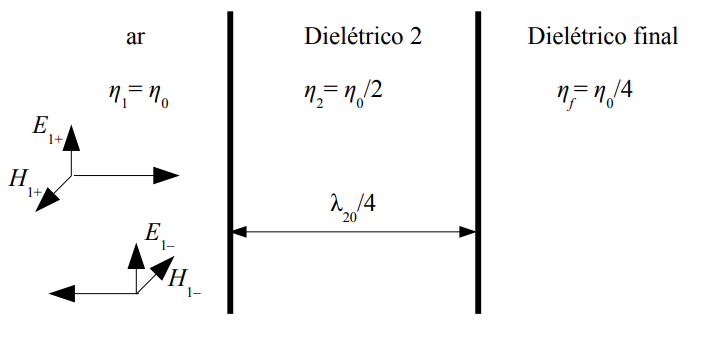
\includegraphics[scale=0.6]{q1.png}

    NUSP: 13683786 $\rightarrow f_0=1,786\ GHz$
\end{center}

\paragraph{a)}

$\epsilon_2=4\ \epsilon_0$

$\ \ d_2 = 20,982\ mm$

\paragraph{b)}

$|\rho_l(f_0-500MHz)|^2=0,092513$

$\ \ |\rho_l(f_0)|^2=7,8\times 10^{-33}\approx 0$

$\ \ |\rho_l(f_0+500MHz)|^2=0,092513$

\break

\begin{center}
    \begin{figure}[h]
    \hspace{-25pt}
    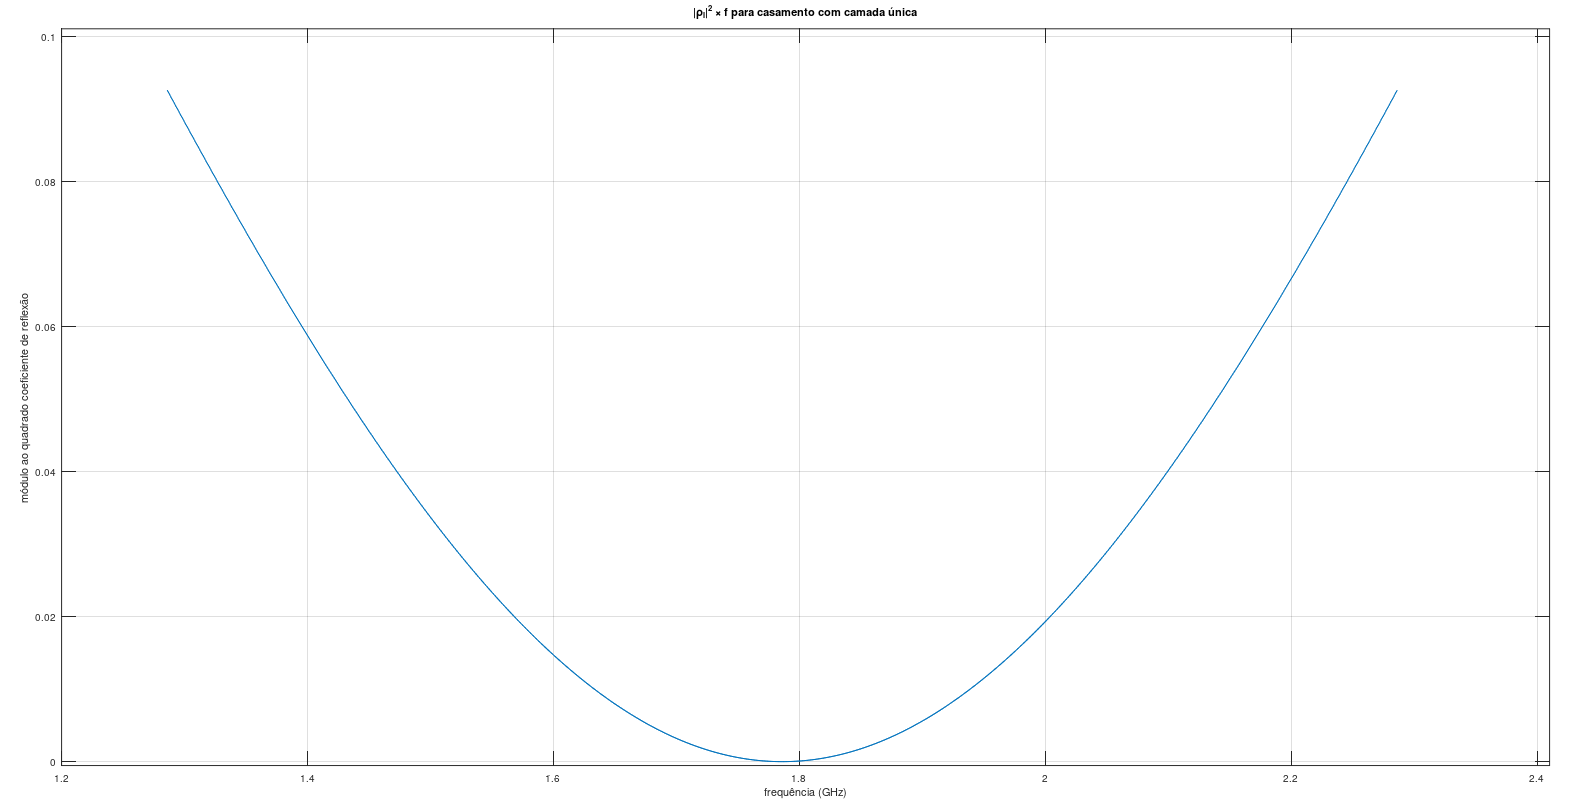
\includegraphics[width=1.1\textwidth]{single.png}

    \caption{Módulo do quadrado do coeficiente de reflexão para uma camada dielétrica}
    \label{fig:awesome_image}
    
    \end{figure}
\end{center}

\vspace{-1cm}

É notável que o casamento planejado funciona muito bem para a frequência determinada, mas que ao se distanciar, o módulo do coeficiente também cresce. Devido ao aumento da quantidade de reflexão que as ondas passam a sofrer dentro do tamanho especificado para o dielétrico, por frequências que passam a se destoar cada vez mais, o comprimento fixado determina então um quadro de descasamento cada vez maior.

\paragraph{c)}

Largura de banda: BW = 94 MHz

Considerando $|\rho_l|^2 \le 0,001:$ Frequências entre 1,739 a 1,833 GHz

%-------------------------------------------
%-------------------------------------------
\newpage
\section{}

\begin{center}
    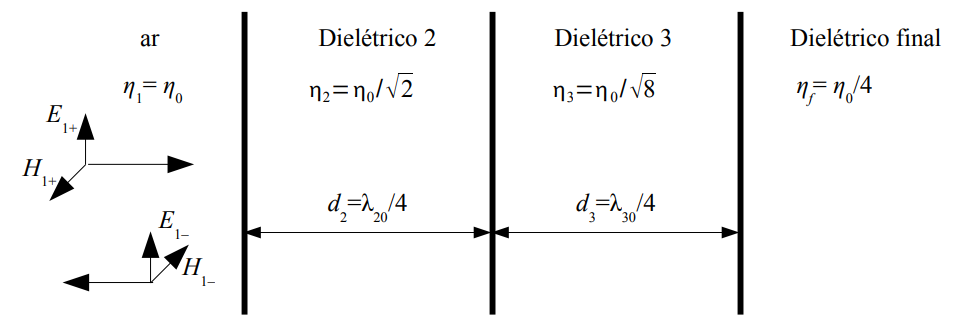
\includegraphics[scale=0.6]{q2.png}
\end{center}

\paragraph{a)}

$\epsilon_2=2\ \epsilon_0$

$\ \ \epsilon_2=8\ \epsilon_0$

$\ \ d_2 = 29,674\ mm$

$\ \ d_3 = 14,837\ mm$

\paragraph{b)}

$|\rho_l(f_0-500MHz)|^2=0,018141$

$\ \ |\rho_l(f_0)|^2=10^{-65}\approx 0$

$\ \ |\rho_l(f_0+500MHz)|^2=0,018141$

\begin{center}
    \begin{figure}[h]
    \hspace{-25pt}
    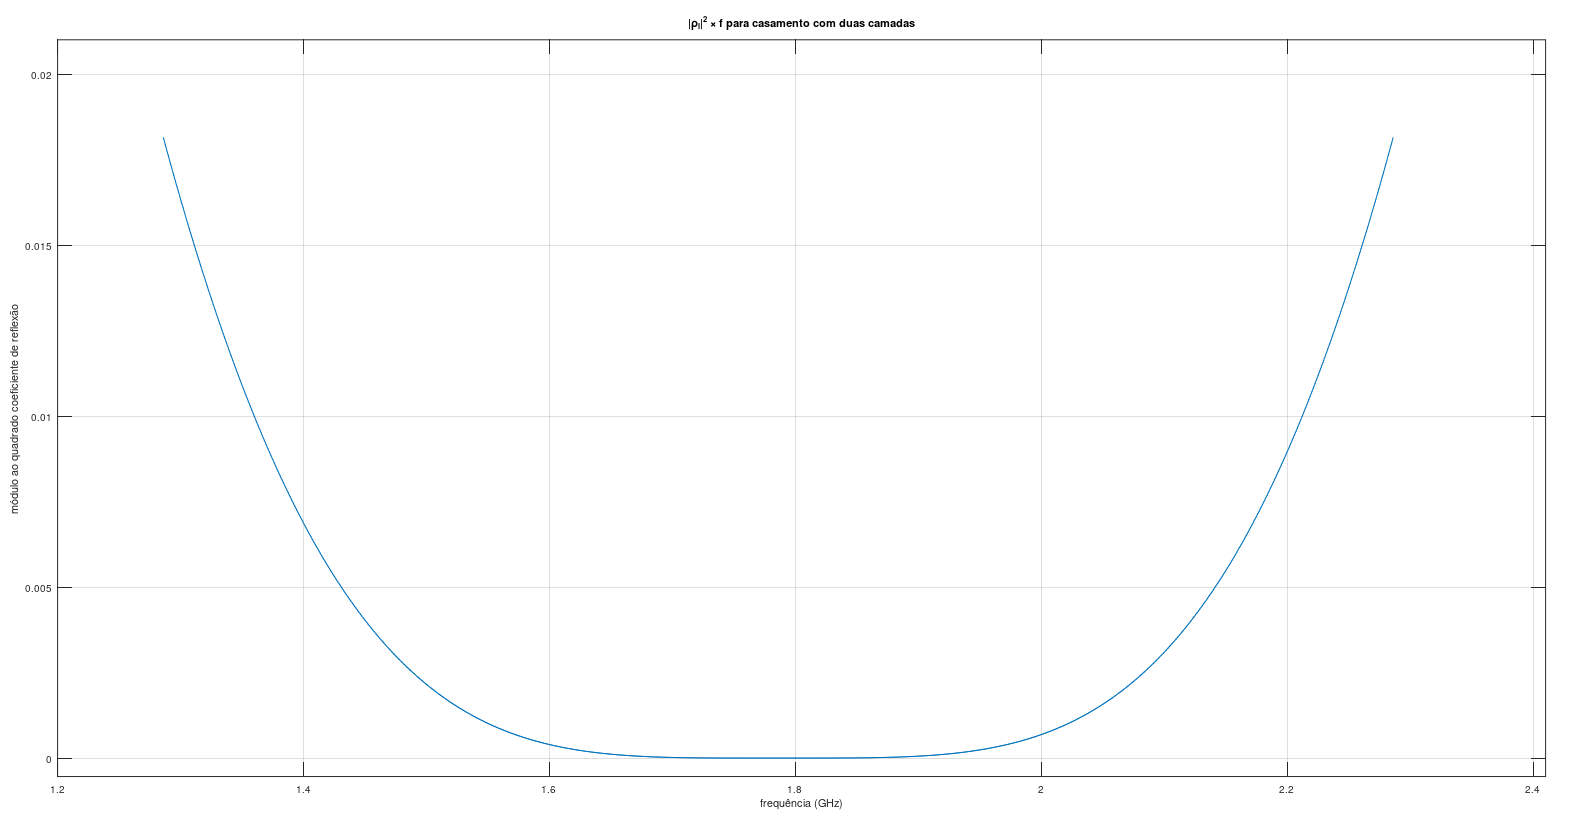
\includegraphics[width=1.1\textwidth]{double.png}

    \caption{Módulo do quadrado do coeficiente de reflexão para duas camadas dielétricas}
    \label{fig:awesome_image_2}
    
    \end{figure}
\end{center}

\vspace{-1.5cm}

\paragraph{c)}

Largura de banda: BW = 470 MHz

Considerando $|\rho_l|^2 \le 0,001:$ Frequências entre 1,551 a 2,021 GHz

\newpage

Ainda que o casamento deste caso também se comporte melhor ao redor da frequência central de especificação para os casamentos dos dielétricos, é notável primeiramente uma região maior em que a reflexão é menor em absoluto, idem pelo formato do gráfico (com uma subida menos acentuada) e pela banda de frequências (5x maior).

Além disso, dentro do mesmo espectro de frequências selecionado, os valores calculados na simulação com dupla camada dielétrica atingiram módulos máximos em valores bem menores que os extremos (nos pontos explicitados de $f_0\ \pm$ 500MHz).

\end{document}